\documentclass{article}

\usepackage{graphicx} % Required for the inclusion of images
\usepackage{amsmath} % Required for some math elements
\usepackage{hyperref}
\usepackage[numbers,sort]{natbib}
\usepackage[russian,english]{babel}
\usepackage[T2A]{fontenc}
\usepackage{placeins}
\usepackage{hyperref}
\usepackage[figurename=Рисунок]{caption}
\usepackage{ dsfont }
\graphicspath{ {./figs/} }
\setlength\parindent{0pt} % Removes all indentation from paragraphs
\renewcommand{\labelenumi}{\alph{enumi}.} % Make numbering in the enumerate environment by letter
\title{Адаптивное и робастное управление \\ Курсовая работа\\ В-1} % Title
\author{Кирилл Лалаянц} % Author name
\date{\today} % Date for the report

\begin{document}

\maketitle % Insert the title, author and date

\begin{center}
\begin{tabular}{l r}
%Date Performed: & January 1, 2012 \\ % Date the experiment was performed
% Выполнили: & Кирилл Лалаянц \\ % Partner names
% &Прокопов Егор \\
Преподаватель: & Герасимов Д.Н. % Instructor/supervisor
\end{tabular}
\end{center}
\newpage
% \begin{abstract}
% Abstract text
% \end{abstract}

\section{Цель работы}

Синтез закона адаптивного управления с использованием метода расширенной ошибки и схемы Лайона, обеспечивающего
ограниченность всех сигналов и слежение выхода объекта за эталонным
сигналом так, чтобы:
\[\lim_{t \rightarrow \infty}(y_M(t) - y(t)) = 0\]
Выход эталонного объекта \(y_M(t)\):
\[y_M(t) = \frac{1}{K_M(s)}[g(t)]=  \frac{1}{s^2 + 5s + 6}[g(t)]\]
Выход объекта \(y(t)\):
\[y(t) = W(s) = \frac{b_0}{s^2 + a_1 s + a_0}[u]\]

Вариант 1: 
\begin{itemize}
  \item \(a_1 = 2\); \(a_0 = -3\);
  \item \(b_0 = 2\);
  \item \(g(t) = 7 \cos(3t + 2) + 8\)
\end{itemize}


\section{Выполнение}
\subsection{Проверка объекта управления на свойства полной управляемости и наблюдаемости.}
\[U = \begin{pmatrix}
  1 & -2 \\
  0 & 2
\end{pmatrix} \rightarrow \text{полностью управляемая}\]
\[V = \begin{pmatrix}
  0 & 1 \\
  2 & 0
\end{pmatrix} \rightarrow \text{полностью наблюдаемая}\]

\subsection{Проверка объекта управления на устойчивость и минимально-фазовость}
Для проверки системы на устойчивость найдем полюса знаменателя её передаточной функции \(W(s)\):
\[\text{pole(W(s)) } = [-3, 1] \rightarrow \text{ неустойчивая и не минимально-фазовая}\]

\subsection{Определение и реализация требуемых компонентов системы}
Выберем фильтры:
\[\dot \nu_1 = \Lambda \nu_1 + e_{n-1}u\]
\[\dot \nu_2 = \Lambda \nu_2 + e_{n-1}y\]
гдe \(e_{n-1} = [0 \hdots 1]^T \in \mathds{R}^{n-1}\); \(\nu_1, \nu_2 \in \mathds{R}^{n-1}\).
\[\Lambda = \begin{bmatrix}
  0 & 1 & \hdots & 0 \\
  \vdots & \vdots & \ddots & \vdots \\
  0 & 0 & \hdots & 1 \\
  -k_0 & -k_1 \hdots & k_{n- 2}
\end{bmatrix} \in \mathds{R}^{(n-1) \times (n-1)} \]

Для данного объекта \(n=2\). Следовательно:
\[\dot \nu_1 = -k_0 \nu_1 + u\]
\[\dot \nu_2 = -k_0 \nu_2 + y\]

Зададим вектора:
\[\omega = [\nu_1^T~\nu_2^T~y]^T\]
\[\omega_p = -[\omega^T~u]^T\]
\[\bar \omega_p = \frac{1}{K_M(s)}[\omega_p]\]
\[\hat{\psi}_p^T = [\hat \psi ~~ \hat b_m] \]

Закон управления:
\[u = \frac{1}{\hat{b}_m}(-\hat{\psi}_p^T \omega + k_0 g(t)) \]

Статическая модель расширенной ошибки:
\[\hat \varepsilon = \bar \omega_p^T \hat{\psi}_p =  \varepsilon - \hat{\psi}_p^T \bar \omega_p + \frac{1}{K_M(s)}[ \hat{\psi}_p^T \omega_p]\]

Градиентный АА:
\[\dot {\hat{\psi}}_p^T = \gamma \Gamma \frac{\bar \omega_p}{1 + \bar \omega_p^T \bar \omega_p} \hat \varepsilon\]
Модифицированный АА:
\[\dot {\hat{\psi}}_p^T = \gamma \Xi^T (\Xi_\varepsilon + \Xi_{\hat{\psi}_p} - \Xi \hat{\psi}_p)\]
\[\Xi = [H_1(s)[\omega]~\dots~H_q(s)[\omega]]^T\]
\[\Xi_\varepsilon = [H_1(s)[\varepsilon]~\dots~H_q(s)[\varepsilon]]^T\]
\[\Xi_{\hat{\psi}_p}  = [H_1(s)[\omega^T \hat{\psi}_p ]~\dots~H_q(s)[\omega^T \hat{\psi}_p ]]^T\]

Гибридный АА:
\[\dot {\hat{\psi}}_p^T = \gamma \Xi^T (\Xi_\varepsilon + \Xi_{\hat{\psi}_p} - \Xi \hat{\psi}_p) + \gamma \Gamma \frac{\bar \omega_p}{1 + \bar \omega_p^T \bar \omega_p} \hat \varepsilon\]
% \begin{figure}[h!]
%   \centering
%   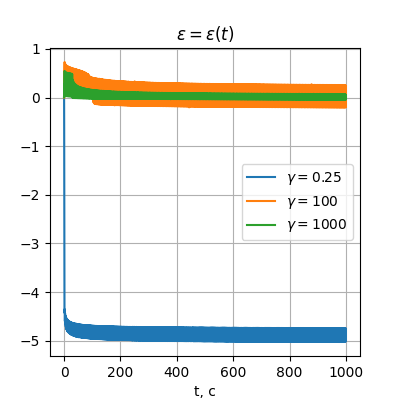
\includegraphics[width=0.65\textwidth]{figs/2_epsilon.png}
%   \caption{График ошибки слежения системы со статической обратной связью.} 
%   \label{fig:2_epsilon}
% \end{figure}


\FloatBarrier



\newpage
\section{Заключение}



\end{document}
